\documentclass{llncs}

\usepackage{listings}
\usepackage{graphicx}
\usepackage{url}

\bibliographystyle{alpha}



\begin{document}

\title{Event-Driven Verification in Dynamic Component Models}

% lets invite Carlos and Birgit - Claas what do you think ??
\author{Jens Dietrich\inst{1} \and Claas Wilke\inst{2}}

\institute{Massey University, Institute of Information Sciences and Technology,\\ Palmerston North, New Zealand \and
Institut f\"ur Software- und Multimediatechnik,\\ Technische Universit\"at Dresden, Germany}

\maketitle



\begin{abstract}

We propose ActiveTreaty, a novel contract and verification model suitable for dynamic component systems. ActiveTreaty combines aspects of static and dynamic verification by checking component contracts whenever certain lifecycle events occur. We introduce a role model that supports the flexible, context-dependent management of different aspects of contract management and enforcement. 
A proof-of-concept implementation for the OSGi/Eclipse component model is presented. 

\end{abstract}



\section{Introduction}

In recent years, dynamic component models supporting the dynamic (re-)configuration of applications have become very successful. Examples include OSGi \cite{OSGI} and its derivatives and .NET \cite{TODO}. Some of the largest and most complex systems are now based on these models, including IBM WebSphere \cite{TODO} and Oracle WebLogic \cite{TODO}. The question arises how these systems can be effectively verified. In practise, static verification techniques are still dominant. This includes the use of compilers and unit testing. Verification is typically performed for single components at built-time. Component containers and runtime environments have little support to verify the integrity of composed systems. For instance, OSGi containers merely check the type safety of classes providing services described by interfaces, and the version compatibility of the components composed. This is based on the implicit assumption that compatibility information between components can be completely described by the combination of service interfaces and dependencies between versioned packages and components. 

In our previous work \cite{Treaty.JOT2009}, we have argued that more expressive contract language is needed to precisely describe the relationship between collaborating components. This has resulted in Treaty, an expressive, component-model independent contract language. Treaty supports alternative contract arrangements (disjunction), collaborations based on resources other than program language types, and therefore contracts that describe different aspects of component compatibility \cite{BeugnardEtAl99} including interface, behavioural and quality of service contracts. It turns out that these features are appropriate to simplify and improve the contract management in application based on dynamic component systems such as Eclipse. 

The original version of Treaty was static in the sense that contracts are represented by integrity rules. Once a contract is instantiated when collaborating components pair up, contracts are ready to be used for verification. However, Treaty makes no assumptions how they are actually used. On the other hand, dynamic component models like OSGi have well defined lifecycle models that describe the various lifecycle states of components, and the transitions between these states. It is therefore possible to use the events signalling state transitions to trigger contract verification. 

In this paper, we propose an extension to make Treaty this dynamic by including both the events that trigger contract verification, and the actions that are to be performed upon verification  to the contracts. This implies that contracts are represented using event-condition-action rules (ECA rules for short). 

The rest of this paper is organised as follows. In the next section, we review related work. We then sketch the Treaty framework. For a detailed description, the reader is referred to \cite{Treaty.JOT2009}. In section 3, we introduce active treaty. TODO:complete 



\section{Related Work}

% TODO Jens: the next two paragraphs are copied from the TKDE submission, need to ve rephrased

To the best of our knowledge our approach is unique in that it addresses the problem of different contract types in dynamic, heterogeneous component models. In \cite{Dong2003}, the authors propose the use of Prolog to express contracts between design components. In contrast to our work, the authors do not consider dynamic and heterogeneous component models. Some authors have explored the possibility of manual and automated contract extraction from Java \cite{Henkel03,MilanovicMalek2004} and .NET programs \cite{ArnoutMeyer2003a}, and the formal representation of these contracts. Arnout and Meyer went on and tried to show the benefits of an a posteriori addition of contracts \cite{ArnoutMeyer2003b}. They set out to resolve the ``closet contract
conjecture'' \cite{ArnoutMeyer2003b}. This conjecture states that there are implicit contracts in software ``lurking under the cover'', and that making
these contract explicit can significantly improve the quality of systems. The intention of this study is very similar to ours. However, the contract language and the nature of the component models analysed are very different. Arnout and Meyer distinguish between ``A Posteriori Contracting'' vs. ``Contracting from the Start''. Treaty goes one step further and supports the combination and aggregations of internal and external contracts. 
%TODO see above 

Semantic web technology has been successfully used to represent contracts in other areas, such as SLA contracts \cite{PaschkeDietrich2005}, business
contracts \cite{Linington04}, \cite{Governatori06} ,\cite{Governatori05} and the provisions for exception handling in electronic contracts \cite{SweetDeal}. These languages are significantly more complex than the Treaty language, and often include features from deontic, temporal or other non-classical logics to gain more expressiveness. The integration of events into the contract logic in some of these approaches is an interesting feature that has great potential for contract-based verification in dynamic component systems. 

\section{Metamodel}




\section{The Treaty Contract Language}

In this section, we provide a brief introduction into Treaty. For more details, the reader is referred to \cite{Treaty.JOT2009}. Treaty is a framework to manage different types of contracts in dynamic component systems. It is based on the idea 
that components interact through connectors by providing and consuming resources. Examples for (dynamic) components are Eclipse plugins and OSGi bundles, examples for connectors are Eclipse extensions and extension points, respectively. Contracts describe this interaction. The requirements in these contracts are themselves expressed through resources that are usually provided by the consumer. Examples for this
are Java interfaces and XML Schemas. Suppliers of services provide other resources that have to have certain typed relationships with consumer side resources. For instance, they provide classes that must \textit{implement} (consumer-side) 
interfaces and XML documents that must \textit{instantiate} XML Schemas. Treaty contracts consist of these typed relationships or boolean expressions built from these relationships. Besides relationships, simple properties (comparisons) and 
resource existence conditions can also be expressed. It turns out that this representation is very appropriate to express many types of contracts in existing component models. In particular in the case of Eclipse,  both logically complex conditions and contracts using resource types other than Java types are indeed required. The type system used by Treaty is based on RDF/OWL \cite{RDF,OWL}. I.e., resource, property and relationship types are represented by URIs and reasoning features such as subtype and subproperty reasoning are supported. 

Treaty is suitable for dynamic component models using late binding since contracts can be defined without explicit reference to a supplier or a consumer. The missing resources can be referenced by function symbols representing 
queries to component meta-data. Once the supplier or consumer is known (at runtime), the contract is instantiated by executing these queries against the component meta data and replacing the functions by the actual resources. 
This process is called \textit{binding}. In the Treaty proof-of-concept implementation for Eclipse, these functions are XPath expressions that are resolved against the \texttt{plugin.xml} meta data file of the supplier plugins when 
binding occurs. 

Figure \ref{fig1} depicts the Treaty model. This model is simplified, in particular, the type hierarchy for Condition representing complex conditions is missing. Treaty supports the a posteriori association of contracts with components. 
This is achieved by using special legislator (contract owner) components that provides contracts for other components.  There are numerous use cases for this, including context-depended contracts and retrofitting existing component-based systems for verification\footnote{see \url{http://www-ist.massey.ac.nz/jbdietrich/treaty/treatyout/index.html} for an experiment where Eclipse has been retrofitted with contracts and verified}.   
 
 

\begin{figure}[t]
\centering
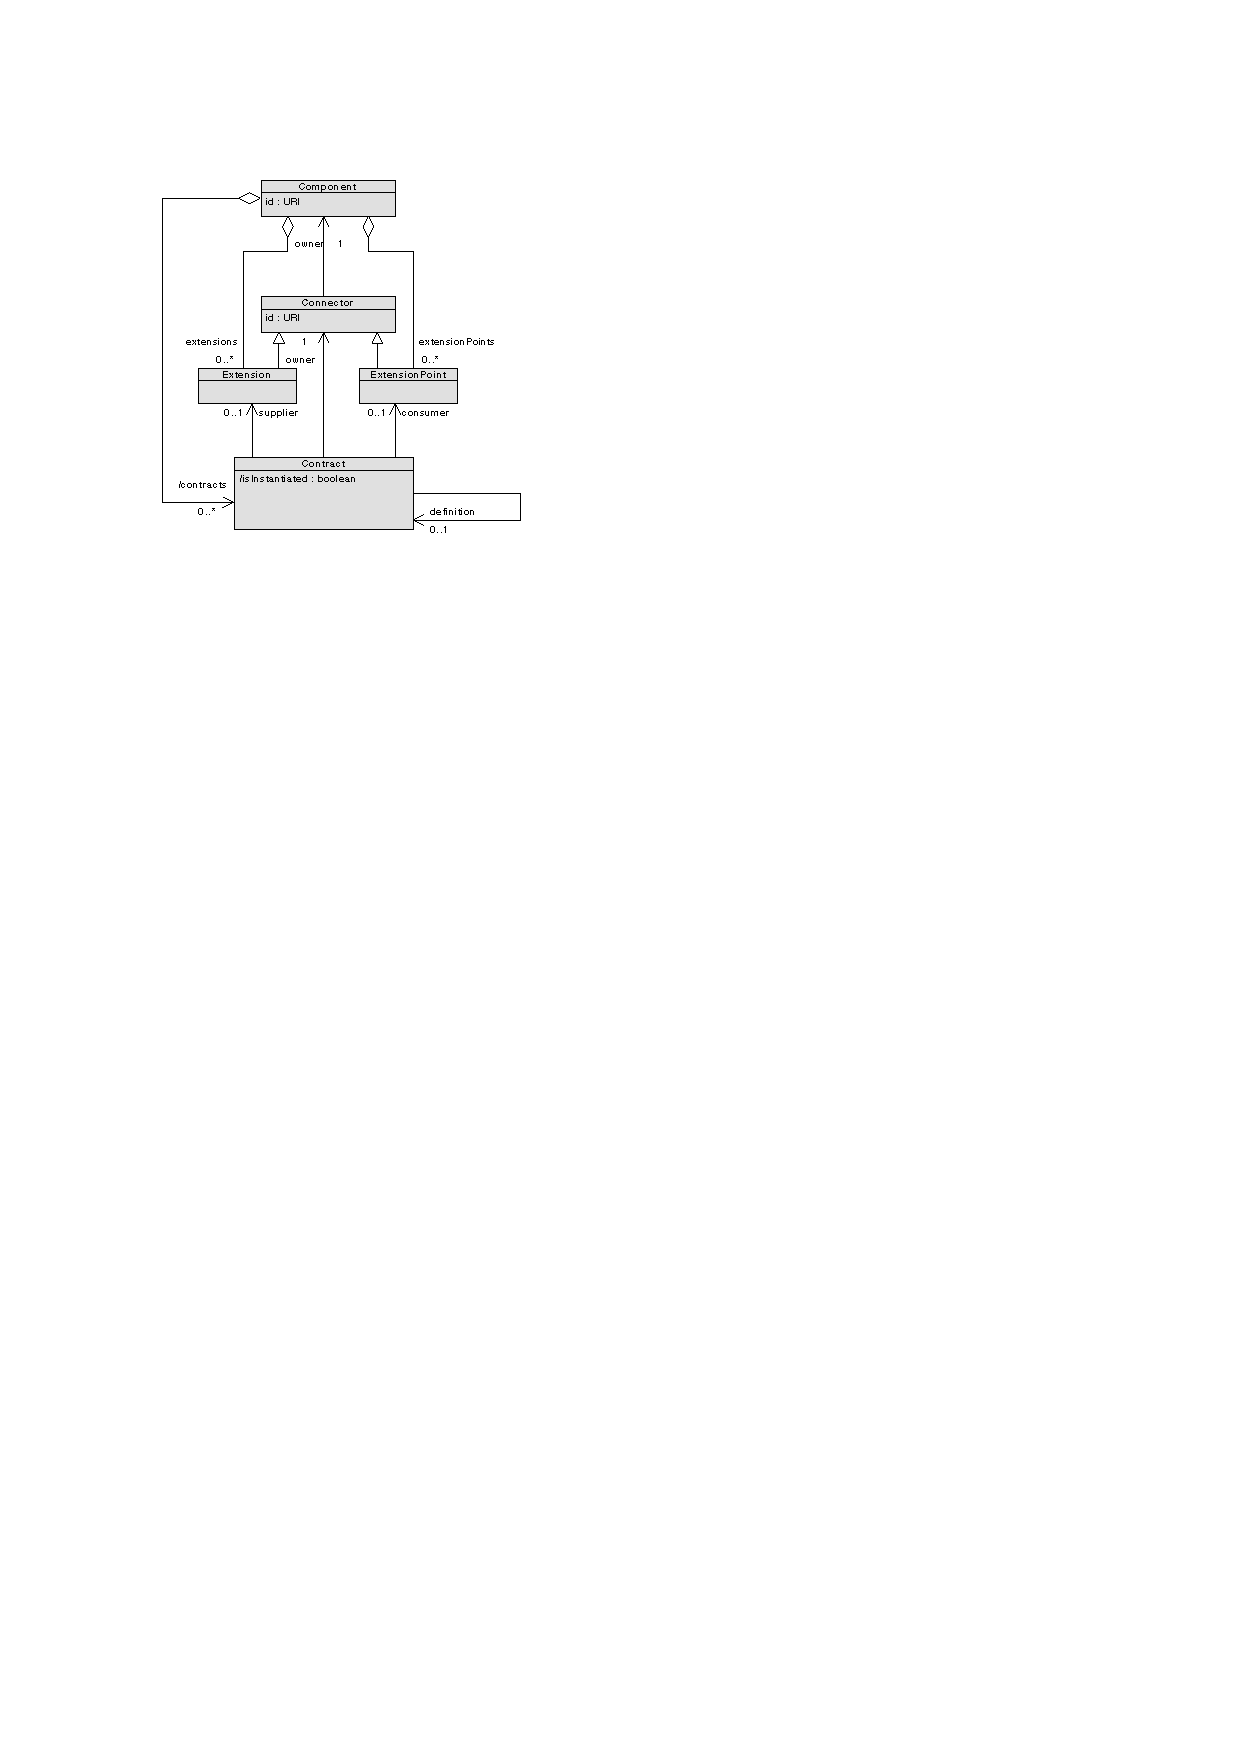
\includegraphics[width=0.5\textwidth]{RoleModel1.pdf}
\caption{Treaty Structure}
\label{fig1}
\end{figure}



\begin{itemize}
\item resources
\item consumers vs suppliers vs legislators
\item contract lifecycle
\item vocabulary contributions
\end{itemize}



\section{Active Treaty}

\begin{figure}[t]
\centering
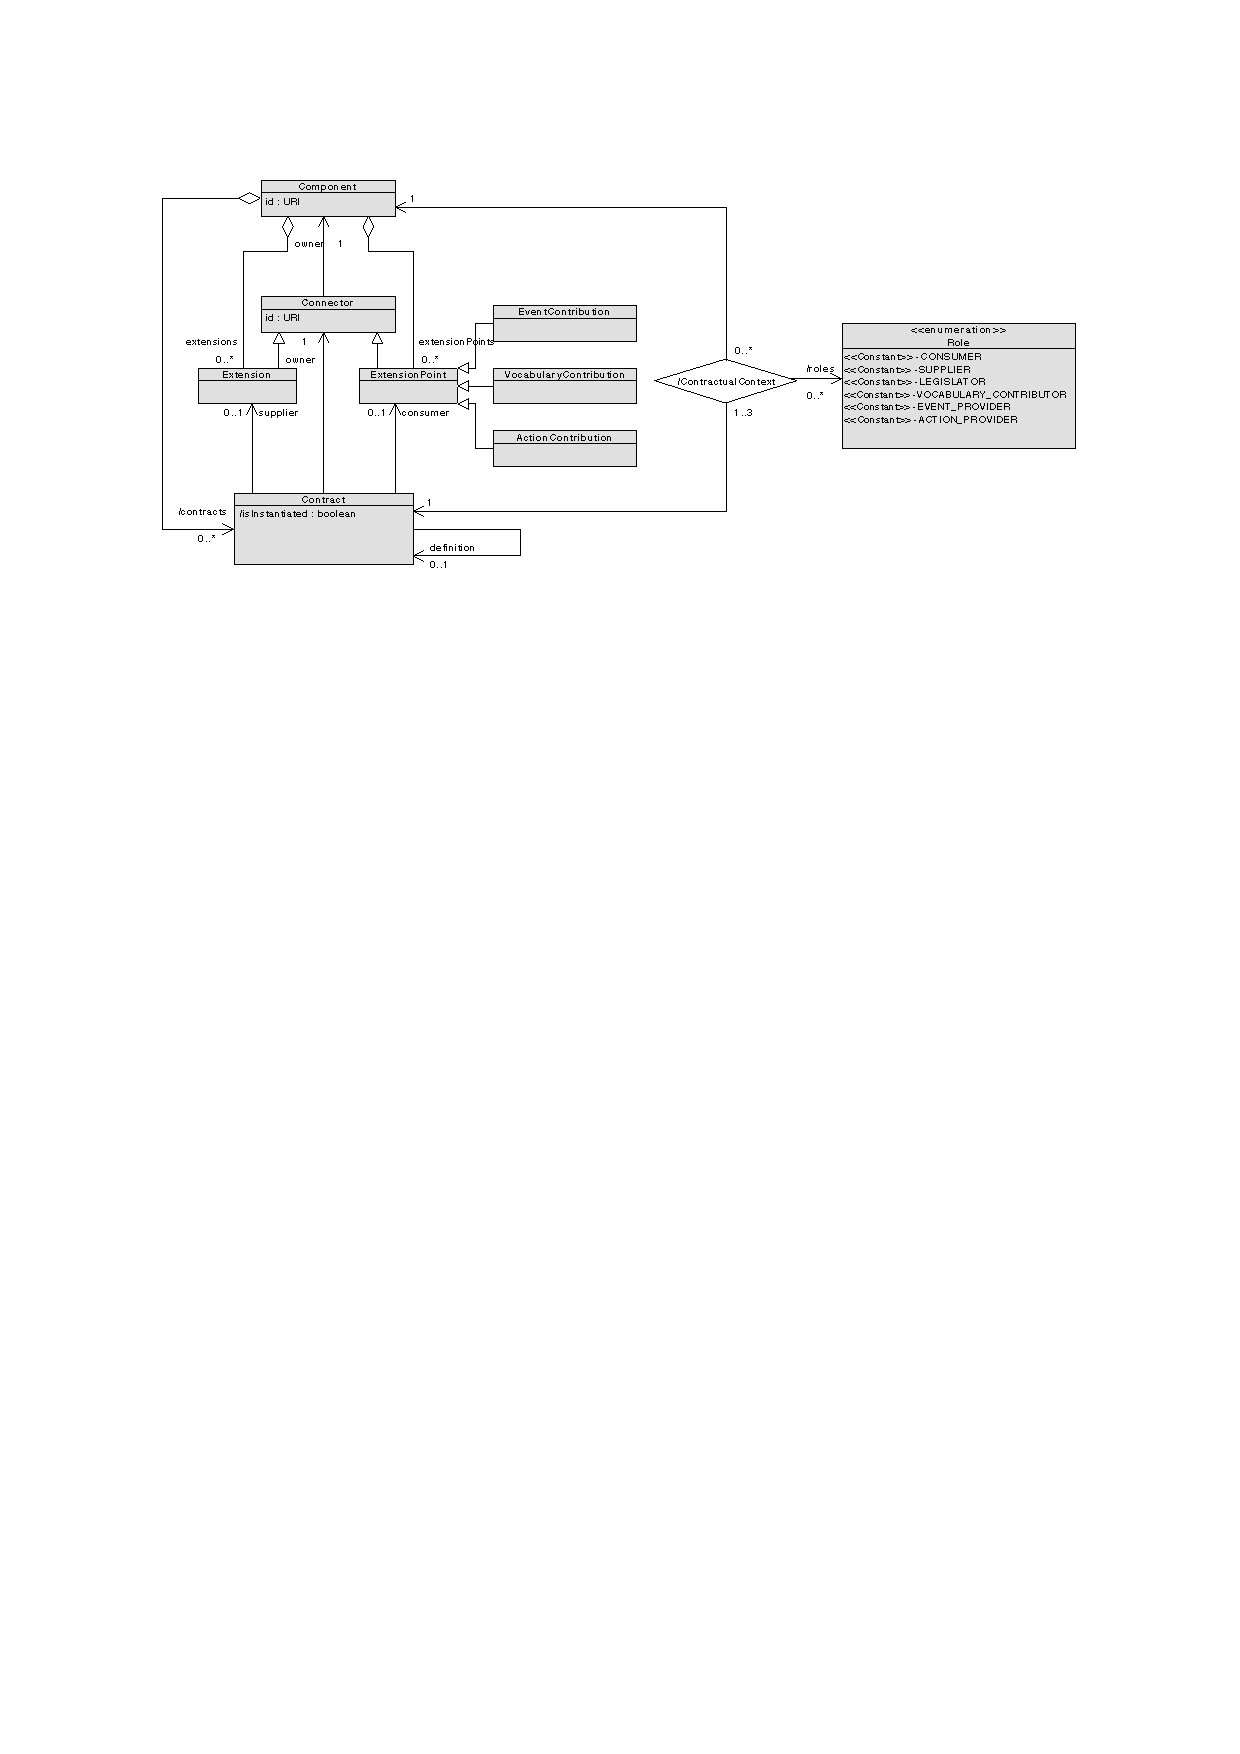
\includegraphics[width=1.0\textwidth]{RoleModel2.pdf}
\caption{Active Treaty and Contract Roles}
\label{fig1}
\end{figure}

\begin{itemize}
  \item dynamic update of contract registry
  \item dynamic update of vocabulary
  \item use (and dynamic update) of trigger and action vocabularies
  \item dynamic verification triggered by triggers
  \item dynamic reaction triggered by verification
\end{itemize}


\subsection{Syntax}

\begin{itemize}
\item EBNF or XML?
\item example
\end{itemize}


\subsection{Semantics}

use event calculus here? or UML activity diagrams



\section{A Role Model for Components}

Consumer
Provider
Legislator - can also be consumer (or supplier, not in Eclipse. E.g., Client/Server)
Vocabulary Contributor



\section{A Case Study: Adding Active Contracts to Eclipse}



\section{Conclusion}


\subsection{Future Works}

\begin{itemize}
	\item support OCL in contracts
	\item implement (Active)Treaty for other component models
\end{itemize}



%TODO change to LNCS style
\bibliography{bibliography}  
    
\end{document}
